\newpage
\setheaders{Panel B}{\daydateyear}
\section{Panel B}
\index{Dunstan, Jocelyn}
\index{Montes y Gomez, Manuel}
\index{Benotti, Luciana}
\index{Perez Rosas, Veronica}

\begin{center}
{\bfseries\Large Perspectivas de NLP desde Latinoam\'erica\\\vspace{2.0\lineskip}NLP perspectives, an overview from Latin America } \\
\vspace{1.0em}
{\large\bf Jocelyn Dunstan, Manuel Montes y Gomez,\\\vspace{2.0\lineskip}Luciana Benotti, and Veronica Perez Rosas } \\

\textbf{\daydateyear{}, 17:00--18:30 CST}\\
\textbf{Do\~na Adelita}
\end{center}


\vspace{1em}
\begin{center}
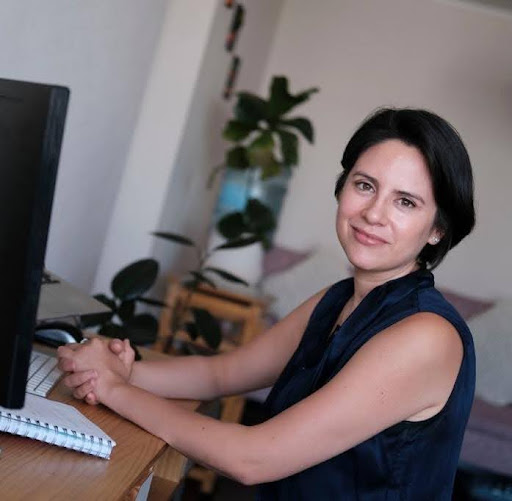
\includegraphics[width=0.3\linewidth]{content/mexican_nlp/jocelyn.jpeg}
\end{center}
{\bfseries Jocelyn Dunstan, Assistant Professor at the Pontifical Catholic University of Chile:}
Jocelyn Dunstan is an Assistant Professor at the Pontifical Catholic University of Chile. She holds a Ph.D.~in Applied Mathematics and Theoretical Physics from the University of Cambridge in the UK. She specializes in leveraging machine learning and natural language processing to address key challenges. Her research primarily revolves around clinical text mining and patient prioritization. In addition to her academic role at the Catholic University of Chile, she is actively engaged as a researcher at prominent institutions such as the Millenium Institute for Foundational Research on Data (IMFD) and the Advanced Center for Electrical and Electronic Engineering (AC3E). Further information about her group's work can be found on their webpage at pln.cmm.uchile.cl.

\vspace{1em}
\begin{center}
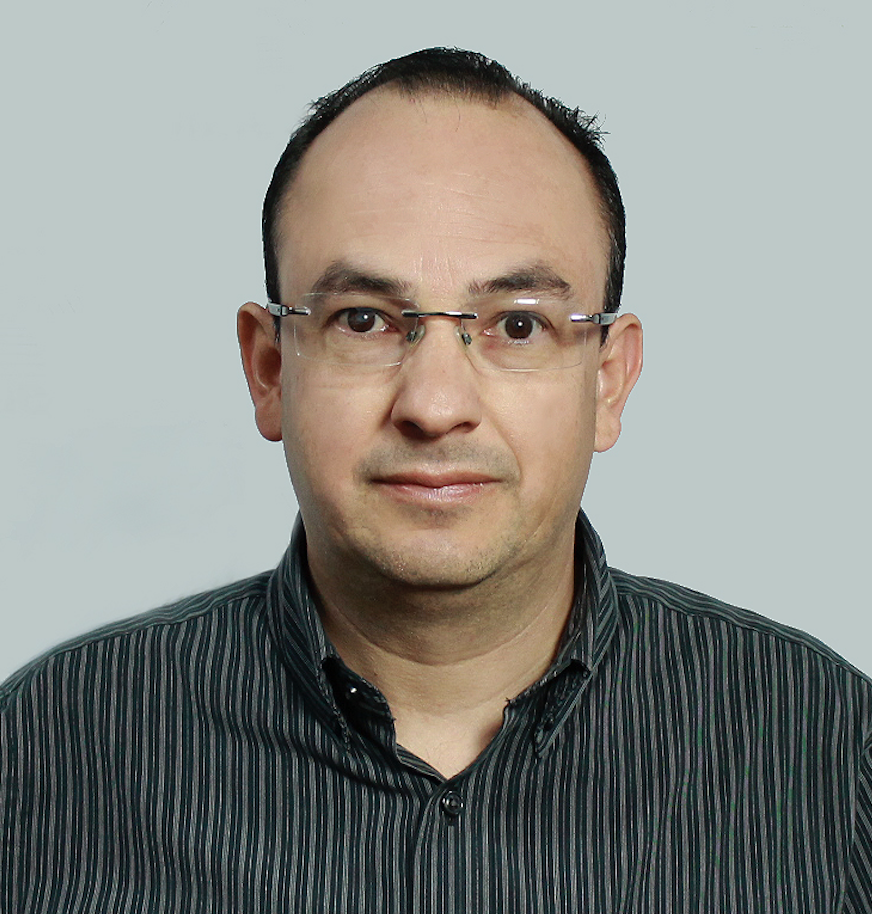
\includegraphics[width=0.3\linewidth]{content/mexican_nlp/manuel.png}
\end{center}.
{\bfseries Manuel Montes y Gomez, Full Professor at National Institute of Astrophysics, Optics and Electronics (INAOE), Mexico:}
Manuel Montes-y-G\'omez is Full Professor at the National Institute of Astrophysics, Optics and Electronics (INAOE) of Mexico. His research is on automatic text processing. He is author of more than 250 journal and conference papers in the fields of information retrieval, text mining and authorship analysis.

He has been visiting professor at the Polytechnic University of Valencia (Spain), and the University of Alabama (USA). He is also a member of the Mexican Academy of Sciences (AMC), and founding member of the Mexican Academy of Computer Science (AMEXCOMP), the Mexican Association of Natural Language Processing (AMNLP), and of the Language Technology Network of CONACYT. In the context of them, he has been the organizer of the National Workshop on Language Technologies (from 2004 to 2016), the Mexican Workshop on Plagiarism Detection and Authorship Analysis (2016-2020), the Mexican Autumn School on Language Technologies (2015 and 2016), and a shared task on author profiling, aggressiveness analysis and fake news detection in Mexican Spanish at IberLEF (2018-2021).

\vspace{1em}
\begin{center}
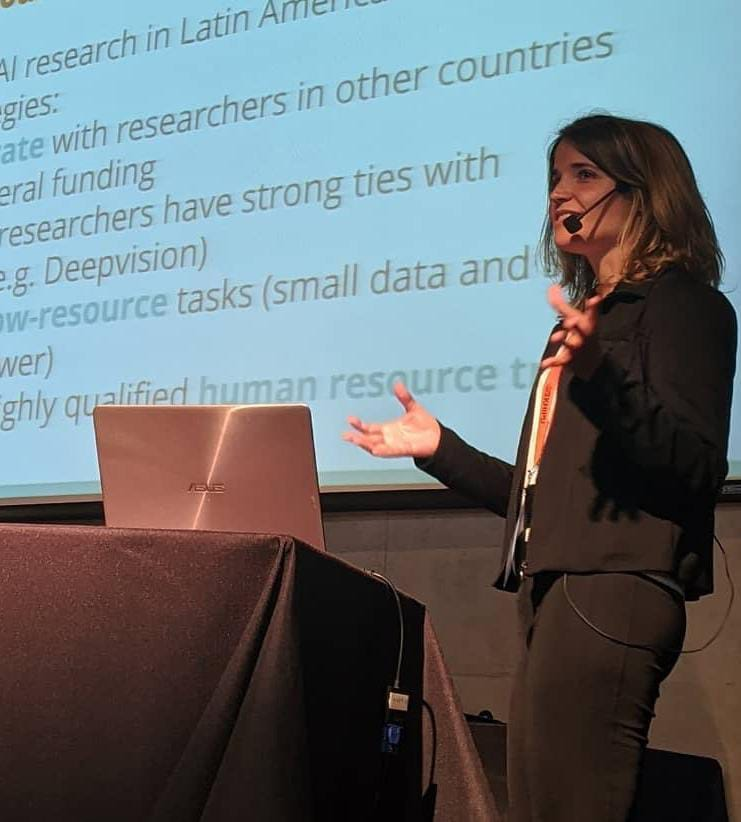
\includegraphics[width=0.3\linewidth]{content/mexican_nlp/luciana.jpg}
\end{center}
{\bfseries Luciana Benotti, Associate Professor at the National University of Córdoba and AI Researcher at CONICET, Argentina:}
Luciana Benotti is an Associate Professor in Computer Science at the National University of C\'ordoba and a Researcher in Artificial Intelligence at CONICET, Argentina. Her research interests include different aspects of situated and interactive NLP, such as interpreting instructions in a dialogue, generating contextualized questions, and deciding when to speak in a dialogue system, among others. She is particularly interested in how linguistic and non-linguistic features contribute to the meaning conveyed during a conversation. These features include what the conversational participants are doing while they talk, the visual context, temporal aspects, etc. She has been a visiting scientist at the University of Trento (2019), Stanford University (2018), Roskilde University (2014), the University of Costa Rica (2012), and the University of Southern California (2010). She holds a joint MSc Erasmus Mundus from the Free University of Bolzano and the Polytechnic University of Madrid and a PhD from the Université de Lorraine. This year, she was chosen as the Latin American representative for the North American Association for Computational Linguistics (NAACL).

\vspace{1em}
\begin{center}
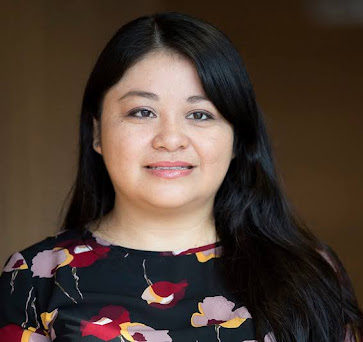
\includegraphics[width=0.3\linewidth]{content/mexican_nlp/veronica.png}
\end{center}
{\bfseries Veronica Perez Rosas, Researcher at the University of Michigan:}
Veronica Perez Rosas obtained her Ph.D.~in Computer Science and Engineering from the University of North Texas in 2014. She is a Level I Researcher recognized by the National System of Researchers. Currently, she is a researcher at the University of Michigan, where she is a part of the Artificial Intelligence laboratory and the Inform Language and Information Technologies research group in the Department of Computer Science. Her research interests include natural language processing (NLP), machine learning, computational linguistics, and multimodal representations. Her research focuses on NLP applications, including automatic detection of misinformation, NLP in mental health, as well as the detection of human behaviors such as sentiment, deception, sarcasm, and affective response.

\newpage
